\section{Physics\-Engine Class Reference}
\label{classPhysicsEngine}\index{PhysicsEngine@{PhysicsEngine}}
{\tt \#include $<$physics\-Engine.hpp$>$}

Collaboration diagram for Physics\-Engine:\begin{figure}[H]
\begin{center}
\leavevmode
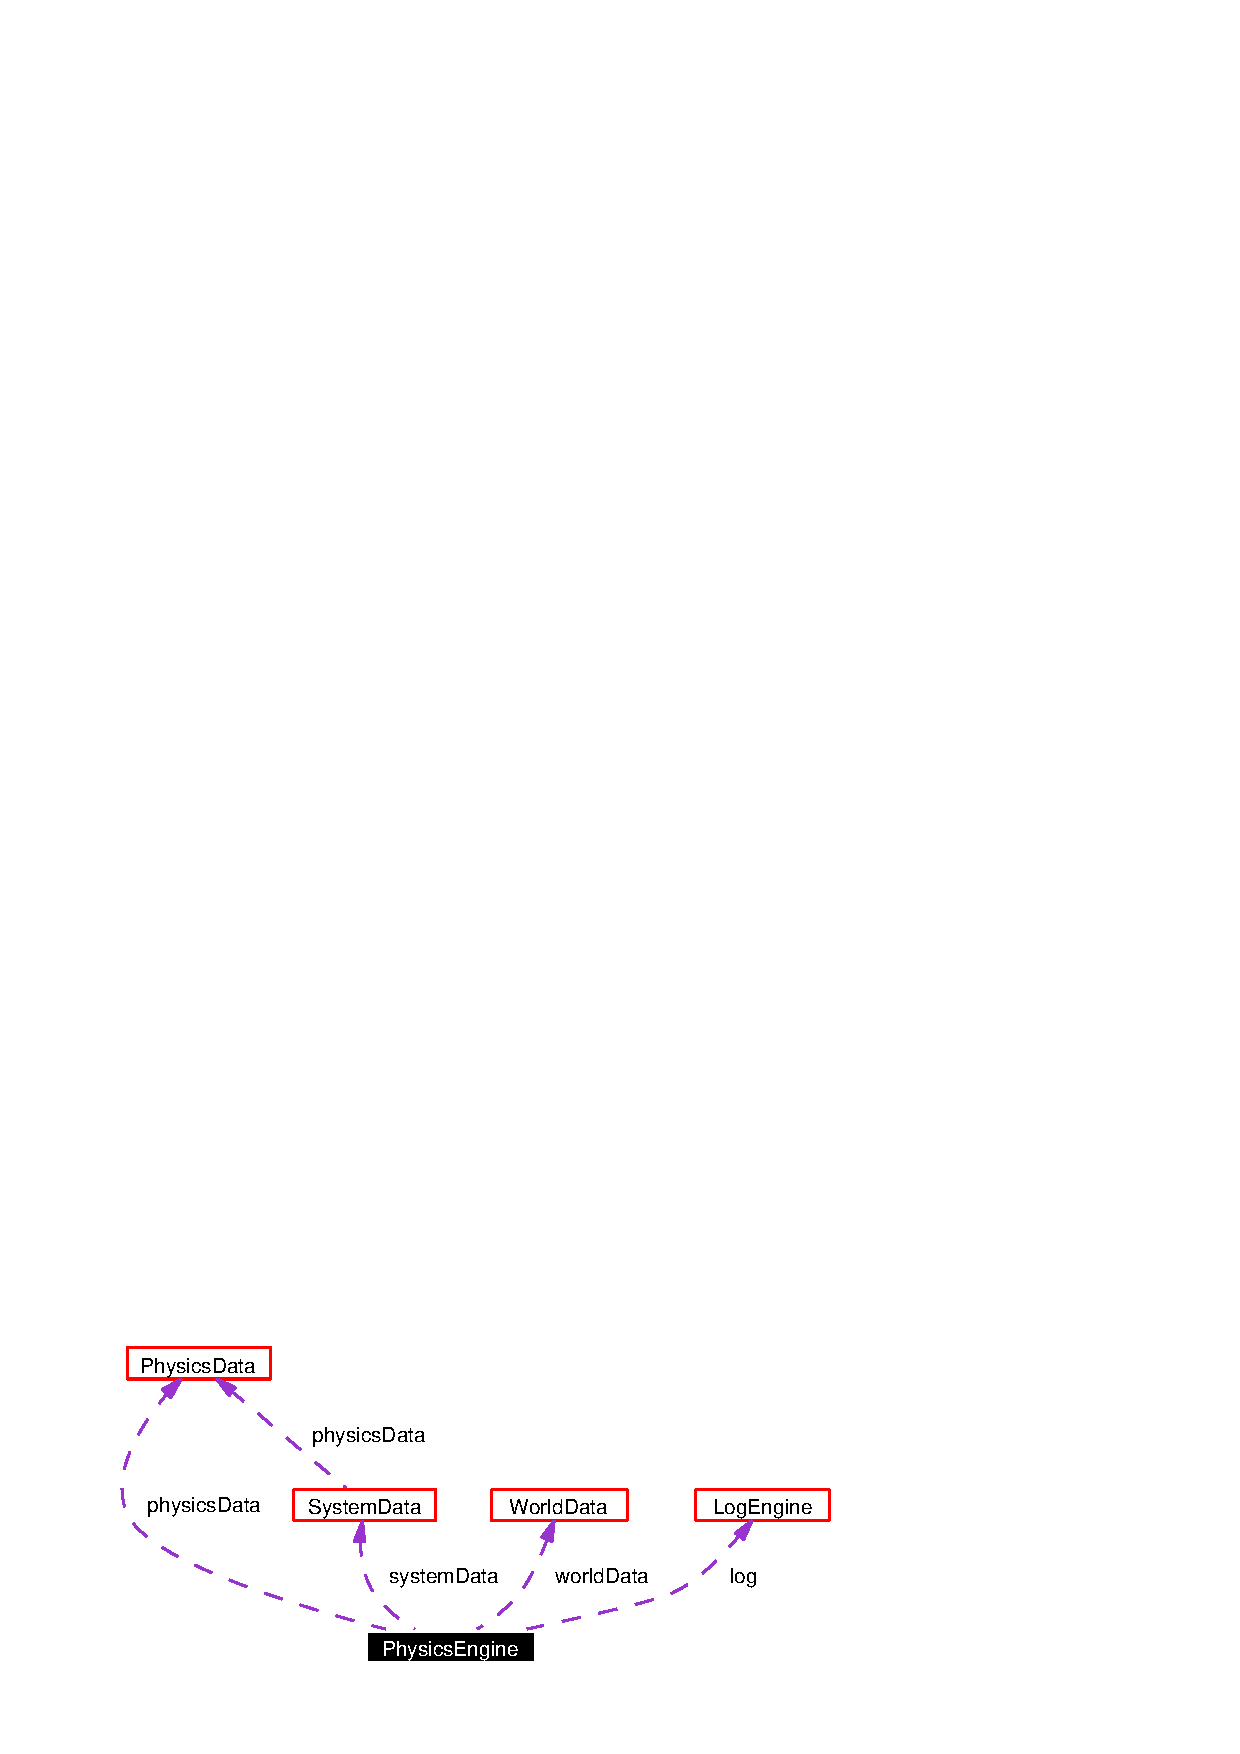
\includegraphics[width=199pt]{classPhysicsEngine__coll__graph}
\end{center}
\end{figure}
\subsection*{Public Member Functions}
\begin{CompactItemize}
\item 
int {\bf start} ({\bf World\-Data} $\ast$wrl\-Data, {\bf System\-Data} $\ast$sys\-Data)
\item 
int {\bf step} (void)
\item 
int {\bf stop} (void)
\end{CompactItemize}
\subsection*{Private Attributes}
\begin{CompactItemize}
\item 
{\bf Log\-Engine} {\bf log}
\item 
{\bf Physics\-Data} $\ast$ {\bf physics\-Data}
\item 
{\bf World\-Data} $\ast$ {\bf world\-Data}
\item 
{\bf System\-Data} $\ast$ {\bf system\-Data}
\end{CompactItemize}


\subsection{Member Function Documentation}
\index{PhysicsEngine@{Physics\-Engine}!start@{start}}
\index{start@{start}!PhysicsEngine@{Physics\-Engine}}
\subsubsection{\setlength{\rightskip}{0pt plus 5cm}int Physics\-Engine::start ({\bf World\-Data} $\ast$ {\em wrl\-Data}, {\bf System\-Data} $\ast$ {\em sys\-Data})}\label{classPhysicsEngine_a0}


\index{PhysicsEngine@{Physics\-Engine}!step@{step}}
\index{step@{step}!PhysicsEngine@{Physics\-Engine}}
\subsubsection{\setlength{\rightskip}{0pt plus 5cm}int Physics\-Engine::step (void)}\label{classPhysicsEngine_a1}


\index{PhysicsEngine@{Physics\-Engine}!stop@{stop}}
\index{stop@{stop}!PhysicsEngine@{Physics\-Engine}}
\subsubsection{\setlength{\rightskip}{0pt plus 5cm}int Physics\-Engine::stop (void)}\label{classPhysicsEngine_a2}




\subsection{Member Data Documentation}
\index{PhysicsEngine@{Physics\-Engine}!log@{log}}
\index{log@{log}!PhysicsEngine@{Physics\-Engine}}
\subsubsection{\setlength{\rightskip}{0pt plus 5cm}{\bf Log\-Engine} {\bf Physics\-Engine::log}\hspace{0.3cm}{\tt  [private]}}\label{classPhysicsEngine_r0}


\index{PhysicsEngine@{Physics\-Engine}!physicsData@{physicsData}}
\index{physicsData@{physicsData}!PhysicsEngine@{Physics\-Engine}}
\subsubsection{\setlength{\rightskip}{0pt plus 5cm}{\bf Physics\-Data}$\ast$ {\bf Physics\-Engine::physics\-Data}\hspace{0.3cm}{\tt  [private]}}\label{classPhysicsEngine_r1}


\index{PhysicsEngine@{Physics\-Engine}!systemData@{systemData}}
\index{systemData@{systemData}!PhysicsEngine@{Physics\-Engine}}
\subsubsection{\setlength{\rightskip}{0pt plus 5cm}{\bf System\-Data}$\ast$ {\bf Physics\-Engine::system\-Data}\hspace{0.3cm}{\tt  [private]}}\label{classPhysicsEngine_r3}


\index{PhysicsEngine@{Physics\-Engine}!worldData@{worldData}}
\index{worldData@{worldData}!PhysicsEngine@{Physics\-Engine}}
\subsubsection{\setlength{\rightskip}{0pt plus 5cm}{\bf World\-Data}$\ast$ {\bf Physics\-Engine::world\-Data}\hspace{0.3cm}{\tt  [private]}}\label{classPhysicsEngine_r2}




The documentation for this class was generated from the following files:\begin{CompactItemize}
\item 
src/physics/{\bf physics\-Engine.hpp}\item 
src/physics/{\bf physics\-Engine.cpp}\end{CompactItemize}
